
\chapter{方法与策略}
\label{chap:methods}

\section{归纳}
\label{sec:induction}

\begin{definition}
  一个命题,若满足以下条件:
  \begin{enumerate}
  \item 存在非负整数$k_0$,命题在$n=k_0$时成立;
  \item 假设命题在$n\le k$时成立可以推出命题在$n=k+1$时成立。
  \end{enumerate}
  则该命题对任意整数$n\ge k_0$都成立。此证明方法称为数学归纳法。
\end{definition}

\begin{example}[求和]
  \begin{align*}
    \frac1{1\times2}+\frac1{2\times3}+\frac1{3\times4}+\cdots+\frac1{n\times (n+1)}
  \end{align*}
\end{example}

可以利用拆项,由$\dfrac1{k\times (k+1)}=\dfrac1k-\dfrac1{k+1}$,从而有
\begin{align*}
  &\frac1{1\times2}+\frac1{2\times3}+\frac1{3\times4}+\cdots+\frac1{(n-1)\times n}\\
  =&\left(\frac11-\frac13\right) + \left(\frac13-\frac14\right) + \cdots + \left(\frac1n-\frac1{n+1}\right)\\
  =&\frac11-\frac1{n+1}\\
  =&\frac{n}{n+1}
\end{align*}

若观察不到拆项的规律,可以考虑一下数学归纳法。记当$n=k$时的和为$S_k$,则
\begin{enumerate}
\item 当$n=1$时,有$S_1=\dfrac12$;
\item 当$n=2$时,有$S_2=\dfrac23$;
\item 当$n=3$时,有$S_3=\dfrac34$;
\item $\cdots$
\end{enumerate}
猜测,$\forall n$,有$S_n=\dfrac{n}{n+1}$。
\begin{proof}
  当$n=1$时,显然成立。

  设当$n\le k$时成立,考虑$n=k+1$的情况。
  \begin{align*}
    S_{k+1}&=S_k + \frac1{(k+1)\times(k+2)}\\
           &=\frac{k}{k+1}+\frac1{(k+1)\times(k+2)}\\
           &=\frac{k(k+2)+1}{(k+1)(k+2)}\\
           &=\frac{k^2+2k+1}{(k+1)(k+2)}\\
           &=\frac{k+1}{k+2}
  \end{align*}
  从而对任意整数$n\ge1$,猜测成立。
\end{proof}



\section{特殊点方法}
\label{sec:special-point-method}

\begin{example}
  求解方程$x\cdot \lfloor x\rfloor=80$,其中$\lfloor x\rfloor$表示不大于$x$的最大整数(向下取整)。
\end{example}
\begin{proof}[解]
  可用猜测法。$x\cdot \lfloor x\rfloor$与$\lfloor x\rfloor ^2$接近,而与$80$最近的完全平方数是$81$,可以考虑$\lfloor x\rfloor=\pm 9$的情况。若$\lfloor x\rfloor=9$,则$x=80/9$,从而$\lfloor x\rfloor=8\ne 9$,矛盾。若$\lfloor x\rfloor=-9$,则$x=-80/9$,这个是吻合的。这种猜测法只是给出了某个解,并没有证明这个解就是所有的解。

  下面是完整解法。由定义,显然有$\lfloor x\rfloor\le x \le \lfloor x\rfloor + 1$。由原题,首先有$x>1$或者$x<-1$。

  \begin{enumerate}
  \item 设$x>1$,则
    \begin{align*}
      \begin{cases}
        \lfloor x\rfloor \cdot \lfloor x\rfloor  \le 80 &\implies \lfloor x\rfloor < 9\\
        \left(\lfloor x\rfloor + 1\right)\cdot \lfloor x\rfloor \ge 80 &\implies \lfloor x\rfloor \ge 9
      \end{cases}
    \end{align*}
    此时无解。
  \item 设$x<-1$,则同样有
    \begin{align*}
      \begin{cases}
        \lfloor x\rfloor \cdot \lfloor x\rfloor  \ge 80 &\implies \lfloor x\rfloor \le -9\\
        \left(\lfloor x\rfloor + 1\right)\cdot \lfloor x\rfloor \le 80 &\implies \lfloor x\rfloor \ge -9
      \end{cases}
    \end{align*}
    此时$\lfloor x\rfloor=-9$,从而$x=-\dfrac{80}{9}$。\qedhere
  \end{enumerate}
\end{proof}


\begin{example}
  已知单位圆上两相互垂直的弦$AB$与$CD$相交于点$M$,则$AB^2+(CM-DM)^2$是常数。

  \centering
  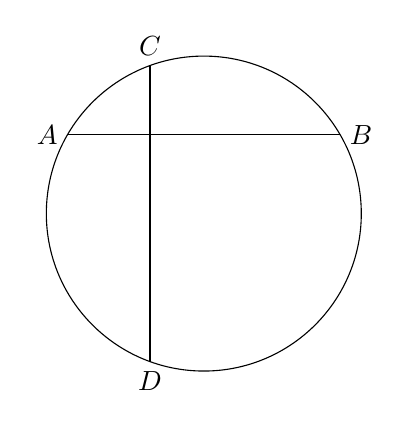
\begin{tikzpicture}[scale=1.0]
    \draw(0,0)circle(2);
    \coordinate[label=right:$B$] (B) at (30:2);
    \coordinate[label=left:$A$] (A) at (150:2);
    \coordinate[label=above:$C$] (C) at (110:2);
    \coordinate[label=below:$D$] (D) at (250:2);
    \tkzInterLL(A,B)(C,D)\tkzGetPoint{M}\tkzLabelPoints[above right](M)
    \tkzMarkRightAngle[color=blue](C,M,A)
    \draw(A)--(B) (C)--(D);
  \end{tikzpicture}
\end{example}
\begin{proof}
  考虑当$AB$与$CD$都是直径的特殊情况,此时$AB=2,CM=DM$,从而有$AB^2+(CM-DM)^2=2^2+0=4$。

  尝试证明对任意两垂直的弦,有$AB^2+(CM-DM)^2=4$。联想勾股定理,需要以$AB$为直角边,直径为斜边作直角三角形,作过点$A$的直径$AE$,则由勾股定理有$AB^2+BE^2=2^2$,从而只再需要证明$BE=|CM-DM|$即可。

  \begin{center}
    \begin{tikzpicture}[scale=1.0]
      \draw(0,0)circle(2);
      \coordinate[label=right:$B$] (B) at (30:2);
      \coordinate[label=left:$A$] (A) at (150:2);
      \coordinate[label=above:$C$] (C) at (110:2);
      \coordinate[label=below:$D$] (D) at (250:2);
      \coordinate[label=below right:$E$] (E) at (330:2);
      \coordinate[label=above right:$O$] (O) at (0,0);
      \tkzDrawPoint(O)
      \tkzInterLL(A,B)(C,D)\tkzGetPoint{M}\tkzLabelPoints[above right](M)
      \tkzMarkRightAngle[color=blue](C,M,A)
      \tkzMarkRightAngle[color=blue](A,B,E)

      \coordinate[label=left:$M'$] (M') at ($(C)!(E)!(D)$);
      \draw(A)--(B)--(E)--cycle (C)--(D);
      \draw[dashed](E)--(M');
      \tkzMarkRightAngle[color=blue](E,M',D)
      \draw[dashed](-3,0)--(3,0)node[pos=0,below]{$L$} node[pos=1,below]{$N$};
    \end{tikzpicture}
  \end{center}

  由上图,只需证明$DM'=CM$即可得到$BE=|DM-CM|$。而这可由对称性,即图形中的相关点关于直线$LN$对称可得。
\end{proof}


\section{构造法}
\label{sec:construction-method}

\begin{example}
  已知$a,b,c$满足方程组
  \begin{align*}
    a+b&=8\\
    ab-c^2+8\sqrt2c&=48
  \end{align*}
  求方程$bx^2+cx-a=0$的根。
\end{example}
\begin{proof}[解]
  变换条件中的方程组的形式,有
  \begin{align*}
    a+b&=8\\
    ab&=c^2-8\sqrt2c+48
  \end{align*}
  以$a,b$为根,构造一元二次方程$(y-a)(y-b)\equiv y^2 - (a+b)y + ab = 0$,即
  \begin{align*}
    y^2 - 8y + (c^2-8\sqrt2c+48) = 0
  \end{align*}
  由于此方程存在两根$a,b$,从而
  \begin{align*}
    & \Delta = (-8)^2 -4(c^2-8\sqrt2c + 48)\ge 0\\
    \implies& c^2-8\sqrt2c + 32\le 0\\
    \implies& \left(c-4\sqrt2\right)^2\le 0\\
    \implies& c=4\sqrt2
  \end{align*}
  从而可解得$a,b$,代入原方程可解得$x$。
\end{proof}


\begin{example}
  若实数$x,y$满足方程组
  \begin{align*}
    \frac{x}{3^3+4^3} + \frac{y}{3^3+6^3} &= 1\\[3pt]
    \frac{x}{5^3+4^3} + \frac{y}{5^3+6^3} &= 1
  \end{align*}
  求$x+y$。
\end{example}
\begin{proof}[解]
  观察原方程组,区别在于$3^3$和$5^3$,把$3^3$和$5^3$看作是以下方程的两个根
  \begin{align*}
    \frac{x}{t+4^3} + \frac{y}{t+6^3} = 1
  \end{align*}
  化简可得
  \begin{align*}
    t^2 - (x+y-4^3-6^3)t - (6^3x + 4^3y - 4^3\cdot 6^3)=0
  \end{align*}
  由韦达定理,有$3^3+5^3=x+y-4^3-6^3$,从而可得$x+y$。
\end{proof}


\section{奇偶分析法}
\label{sec:even-odd-method}

\begin{example}
  能否用下面5种图形各一个拼成一个$4\times5$的长方形?

  \centering
  \begin{tikzpicture}[scale=.5]
    \draw(0,0)grid(1,3)grid(2,2);
    \draw(3,0)grid(5,2);
    \draw(6,0)grid(7,4);
    \draw(8,0)grid(10,1) (9,1)grid(11,2);
    \draw(12,0)grid(15,1) (13,1)grid(14,2);

    \begin{scope}[shift={(5,-5)}]
      \draw(0,0)grid(5,4);
    \end{scope}
  \end{tikzpicture}
\end{example}
\begin{proof}[解]
  将$4\times5$的图形如棋盘般染色,如下图。
  \begin{center}
    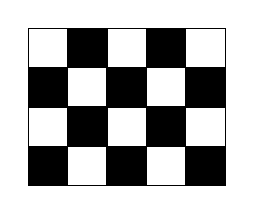
\begin{tikzpicture}[scale=.5]
      \draw(0,0)grid(5,4);
      \fill(0,0)rectangle(1,1)
           (0,2)rectangle(1,3)
           (1,1)rectangle(2,2)
           (1,3)rectangle(2,4)
           (2,0)rectangle(3,1)
           (2,2)rectangle(3,3)
           (3,1)rectangle(4,2)
           (3,3)rectangle(4,4)
           (4,0)rectangle(5,1)
           (4,2)rectangle(5,3);
    \end{tikzpicture}
  \end{center}
  则无论如何摆放,前4种图形都会覆盖两个白格子两个黑格子,最后一种图形\tikz[scale=.25]{\draw(0,0)grid(3,1)(1,1)grid(2,2);}都会覆盖奇数个白格子奇数个黑格子(一个白格子加三个黑格子,或者三个白格子加一个黑格子)。按奇偶性,5种图形各一个,无法覆盖偶数个白格子和偶数个黑格子。
\end{proof}

\begin{example}
  若$a_1,a_2,a_3,\cdots,a_7$是$1,2,3,\cdots,7$这$7$个数的一个排列,则
  \begin{align*}
    P\equiv (a_1 - 1)(a_2-2)\cdots(a_7-7)
  \end{align*}
  是偶数。
\end{example}
\begin{proof}
  反证。若$P$是奇数,则$a_1-1, a_2-2, a_3-3,\cdots, a_7-7$都是奇数,从而其和也是奇数。然而$a_1,a_2,\cdots,a_7$是$1,2,\cdots,7$的排列,从而其和$(a_1-1) + (a_2-2) + \cdots + (a_7-7)=(a_1+a_2+\cdots + a_7)-(1+2+\cdots+7)=0$应为偶数。矛盾。
\end{proof}

\begin{example}
  在区间$(1,\sqrt2)$内任取$n$个点,按大小顺序记为$x_1,x_2,\cdots,x_n$,再加上$x_0=1$,$x_{n+1}=\sqrt2$
\end{example}

\section{假设}
\label{sec:assumption}

\begin{example}[鸡兔同笼]
  一个笼子里着好多鸡和兔子。上面看去,可以数到有10个头,从下面看去,可以数到有28只脚。问笼子里有几只鸡几只兔子?
\end{example}
\begin{proof}[提示]
  这个用方程来说显然是非常简单的。若用假设法的话,则更直观。

  假设笼子里的全是鸡,那10个头就是10个鸡,总共应该有$10\times2=20$只脚。现在多了$28-20=8$只脚,只能是假设的10个鸡里有几个应该要换成兔子。而每1个鸡换成1个兔子,脚的总数就会多$4-2=2$只,所以应该是$8\div 2=4$只鸡要换成兔子。即兔子有$4$只,鸡有$10-4=6$只。

  若假设全是兔子,也可以用类似的分析方法得到相同的答案。
\end{proof}